\documentclass[10pt]{beamer}

\usetheme{metropolis}
\usepackage{appendixnumberbeamer}

\usepackage{booktabs}
\usepackage[scale=2]{ccicons}
\usepackage{graphicx}
\usepackage{hyperref}
\usepackage{circuitikz}
\usepackage{pdflscape}
\usepackage{smartdiagram}

\usepackage{color}
\usepackage{listings}

\lstset{
	basicstyle=\footnotesize\ttfamily,
    keepspaces=true,
    showstringspaces=false,
    language=PHP,
    commentstyle=\ttfamily,
}

\usepackage[OT4]{polski}
\usepackage[utf8]{inputenc}

\usepackage{pgfplots}
\usepgfplotslibrary{dateplot}

\usepackage{xspace}
\newcommand{\themename}{\textbf{\textsc{metropolis}}\xspace}

\setbeamertemplate{frame footer}{}
\setbeamertemplate{frame numbering}{}

\usetikzlibrary{shapes,arrows}

\tikzstyle{decision} = [diamond, draw, fill=blue!20, 
    text width=4.5em, text badly centered, node distance=3cm, inner sep=0pt]
\tikzstyle{block} = [rectangle, draw, fill=blue!20, 
    text width=5em, text centered, rounded corners, minimum height=4em]
\tikzstyle{line} = [draw, -latex']
\tikzstyle{cloud} = [draw, ellipse,fill=red!20, node distance=3cm,
    minimum height=2em]


\title{Mapowanie relacyjno-obiektowe}

\subtitle{Projektowanie i programowanie systemów internetowych I}
\author{mgr inż. Krzysztof Rewak}
\date{\today}
\institute{Wydział Nauk Technicznych i Ekonomicznych \\ Państwowa Wyższa Szkoła Zawodowa im. Witelona w Legnicy}

\begin{document}

\maketitle

\begin{frame}{Plan prezentacji}
  \setbeamertemplate{section in toc}[sections numbered]
  \tableofcontents[hideallsubsections]
\end{frame}


\section{Bazy danych w aplikacjach webowych}

\begin{frame}[fragile]{Operacje na bazach danych}
	\begin{lstlisting}	
$connection_string = "mysql:host=localhost;dbname=db";
$user = "root";
$password = "";

$pdo = new \PDO($connection_string, $user, $password);
$users = $pdo->query("SELECT * FROM users;");

foreach($users as $user) {
    echo $user;
}
	\end{lstlisting}
\end{frame}

\begin{frame}[fragile]{Operacje na bazach danych}
	\begin{lstlisting}
import MySQLdb as m

host = "localhost"
user = "root"
password = ""
db = "db"

db = m.connect(host=host, user=user, passwd=password, db=db)

cursor = db.cursor()
cursor.execute("SELECT * FROM users;")

users = cursor.fetchall()

for user in users:
    print user
    
db.close()
	\end{lstlisting}
\end{frame}

\begin{frame}[fragile]{Operacje na bazach danych}
	\begin{lstlisting}
var connection = InitalizeConnectionToDb();
var select = new SelectBD();

select.Open(connection, @"SELECT * FROM Users");
foreach(var user in select.DataTable)
{
    Console.WriteLine(user);
}

	\end{lstlisting}
\end{frame}

\begin{frame}{Operacje na bazach danych}
	Czy można zbudować wielki system internetowy korzystając z prostego wypisywania kwerend, wysyłania ich do bazy danych i interpretacji wyników?
	
	\ \\
\end{frame}

\begin{frame}{Operacje na bazach danych}
	Czy można zbudować wielki system internetowy korzystając z prostego wypisywania kwerend, wysyłania ich do bazy danych i interpretacji wyników?
	
	Oczywiście, że można.
\end{frame}

\begin{frame}{Operacje na bazach danych}
	Czy można sensownie zbudować wielki system internetowy korzystając z prostego wypisywania kwerend, wysyłania ich do bazy danych i interpretacji wyników?
	
	\ \\
\end{frame}

\begin{frame}{Operacje na bazach danych}
	Czy można sensownie zbudować wielki system internetowy korzystając z prostego wypisywania kwerend, wysyłania ich do bazy danych i interpretacji wyników?
	
	Może niekoniecznie.
\end{frame}

\begin{frame}{Operacje na bazach danych}	
	\texttt{SELECT content FROM disadvantages;}
	
	Wady korzystania z ręcznego budowania zapytań:
	
	\begin{itemize}
		\item redundancja kodu;
		\item brak kontroli na spójnością systemu;
		\item problemy przy zmianach koncepcji;
		\item wymóg poznania przynajmniej dwóch języków programowania?
	\end{itemize}
\end{frame}

\section{Mapowanie z relacji na obiekty}

\begin{frame}[fragile]{Uproszczony schemat działania ORM}
	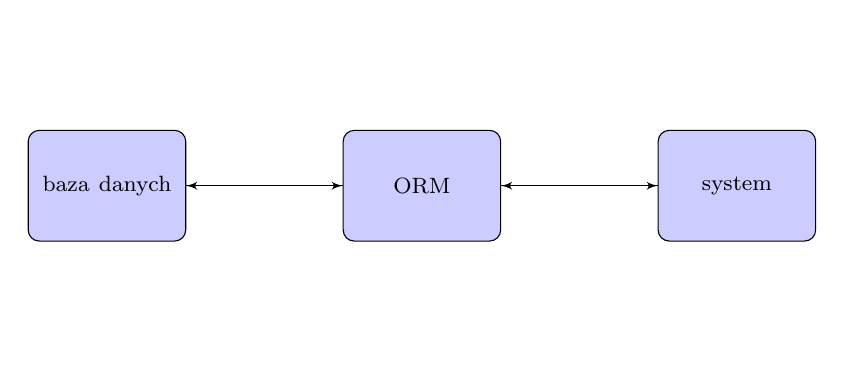
\begin{tikzpicture}[node distance=4cm, minimum size=2cm, auto]
		\node [block] (db) {\footnotesize baza danych};
		\node [block, right of=db] (orm) {\footnotesize ORM};
		\node [block, right of=orm] (code) {\footnotesize system};
		
		\path [line] (db) edge node {} (orm);
		\path [line] (orm) edge node {} (code);
		\path [line] (code) edge node {} (orm);
		\path [line] (orm) edge node {} (db);
	\end{tikzpicture}
\end{frame}

\begin{frame}[fragile]{Spaghetti code}
	\begin{lstlisting}	
$query = "SELECT id, login, email
          FROM users
          WHERE id = 1;
          ";

$result = $pdo->query($query);
	\end{lstlisting}
\end{frame}

\begin{frame}[fragile]{Spaghetti code}
	\begin{lstlisting}	
$query = "SELECT users.id, login, email, birthdate
          FROM users
          JOIN profiles
              ON profiles.id = users.id
          WHERE users.id = 1;
          ";

$result = $pdo->query($query);
	\end{lstlisting}
\end{frame}

\begin{frame}[fragile]{Lepiej?}
	\begin{lstlisting}	
User::with("profiles")->find(1);
	\end{lstlisting}
\end{frame}

\begin{frame}{Co warto zapamiętać?}	
	ORM jest systemem mapującym - a więc tłumaczącym - bazodanowe tabele i relacje na model obiektowy. 
	
	\textbf{Nie jest to w żadnym wypadku obiektowa baza danych}, a jedynie sposób, aby wykorzystać nieobiektową bazę w obiektowy sposób.
\end{frame}

\begin{frame}{Zalety}	
	Dlaczego warto korzystać z mapowania relacyjno-obiektowego?
\end{frame}

\begin{frame}{Spójność danych}
	Zaleta: Odpowiednio zamodelowane dane będą spójne względem siebie i systemu.
\end{frame}

\begin{frame}{Spójność danych}	
	Przykład: klient ma sklep internetowy. Jak wprowadzić do działającego już systemu kilka walut, bo klient chce wejść na rynek międzynarodowy?
\end{frame}

\begin{frame}{Spójność danych}	
	Jedno z rozwiązań: przepisać wszystkie zapytania na joiny do tabeli walut.
	
	Jedno z rozwiązań: zmienić metodę pobierania produktów w modelu na pobieranie z połączeniem do walut i ewentualnym ustawieniem waluty domyślnej.
\end{frame}

\begin{frame}{Separacja warstw}
	Zaleta: Można oddzielić warstwę logiki biznesowej od warstwy zapisanych danych.
\end{frame}
	
\begin{frame}{Separacja warstw}	
	Przykład: klient ma system do zarządzania przedsiębiorstwem. Jak sensownie oddzielić dane pracowników obecnie pracujących od tych, którzy już nie pracują?
\end{frame}
	
\begin{frame}{Separacja warstw}
	Jedno z rozwiązań: stworzyć dwie tabele \texttt{active\_employees} i \texttt{nonactive\_employees} lub dodać kolumnę \texttt{is\_active} do łączonej tabeli \texttt{employees}.
	
	Jedno z rozwiązań: stworzyć modele \texttt{ActiveEmployee}, \texttt{NonactiveEmployee} i \texttt{Employee}, które będą bazowały na jednej tabeli.
\end{frame}

\begin{frame}{Zależności technologiczne}
	Zaleta: Można uniezależnić się od technologii bazodanowej.
\end{frame}
	
\begin{frame}{Zależności technologiczne}	
	Przykład: klient ma system do zarządzania budżetem. Okazuje się, że jego silnik bazy danych ma w sobie krytyczny błąd bezpieczeństwa, więc trzeba relatywnie bezkosztowo zmienić DBMS. Co robić?
\end{frame}
	
\begin{frame}{Zależności technologiczne}	
	Jedno z rozwiązań: przepisać dosłownie wszystko.
	
	Jedno z rozwiązań: zmienić wartość jednej zmiennej konfiguracyjnej.
\end{frame}

\begin{frame}{Zalety}	
	Więcej zalet?
	
	\begin{itemize}
		\item większa kontrola nad kodem,
		\item praca nad konkretnymi obiektami, a nie abstrakcyjnymi tablicami, 
		\item możliwość podpięcia obserwatorów/zdarzeń,
		\item możliwość podpięcia systemu cache'ującego,
		\item wiele innych. 
	\end{itemize}
\end{frame}

\section{Wzorce}
	
\begin{frame}{Jak ugryźć ORM?}	
	Warto omówić przynajmniej dwa podstawowe podejścia do mapowania relacyjno-obiektowego. Oba wykorzystują wzorce architektoniczne: kolejno \emph{active record} i \emph{data mapper}.
\end{frame}
	
\begin{frame}{Aktywny rekord}
	\emph{Aktywny rekord} to - uogólniając - pomysł wedle którego każdy obiekt wykorzystywany przez ORM jest wyposażony w najważniejsze funkcjonalności.
\end{frame}

\begin{frame}[fragile]{Aktywny rekord}
	Każdy obiekt powinien dziedziczyć po nadrzędnej klasie \emph{modelu}, która umożliwi pracę w formie aktywnego rekordu. 
	
	Przykładowy model najprostszego produktu sklepowego może wyglądać następująco:

	\begin{lstlisting}	
class Product(models.Model):
    name = models.CharField(max_length=64)
    price = models.DecimalField()
	\end{lstlisting}
\end{frame}

\begin{frame}[fragile]{Aktywny rekord}
	Klasę modelu można wówczas wykorzystać między innymi do tworzenia obiektów i zapisywania ich w bazie danych:
	
	\begin{lstlisting}	
product = Product(name="Inifinity Gauntlet", price=99.90)
product.save()
	\end{lstlisting}
\end{frame}

\begin{frame}[fragile]{Aktywny rekord}
	Klasa modelu może też służyć jako źródło do pobierania obiektów z bazy:
	
	\begin{lstlisting}	
products = Product.objects.all()

for product in products:
    print product
	\end{lstlisting}
\end{frame}

\begin{frame}[fragile]{Aktywny rekord}
	Klasa modelu może też służyć jako źródło do pobierania obiektów z bazy:
	
	\begin{lstlisting}	
products = Product.objects.filter(price__lte=100)

for product in products:
    print product
	\end{lstlisting}
\end{frame}

\begin{frame}[fragile]{Aktywny rekord}
	Przykładowo można usunąć wszystkich użytkowników, którzy nie aktywowali się przeciągu tygodnia od rejestracji:
	
	\begin{lstlisting}	
from datetime import datetime, timedelta

threshold = datetime.today() - timedelta(days=7)

users = User.objects.filter(created_at__lte=threshold,
                            is_active=False)

for user in users:
    user.delete()
    
# OR users.delete()
	\end{lstlisting}
\end{frame}

\begin{frame}[fragile]{Aktywny rekord}
	Zalety?
	\begin{itemize}
		\item wszystko jest \emph{pod ręką},
		\item początkowo może się wydawać bardziej intuicyjny.
	\end{itemize}
	
	Wady?
	\begin{itemize}
		\item ciężkie modele,
		\item brak separacji warstw.
	\end{itemize}
\end{frame}
	
\begin{frame}{Konwerter danych}
	\emph{Konwerter danych} to - uogólniając - pomysł wedle którego każdy obiekt wykorzystywany przez ORM jest jedynie reprezentacją danych, a funkcjonalnościami zajmuje się osobna warstwa.
\end{frame}

\begin{frame}[fragile]{Konwerter danych}
	Obiekt to tylko i wyłącznie rozpisane dane:

	\begin{lstlisting}	
class Product():
    name = None
    price = None
	\end{lstlisting}
\end{frame}

\begin{frame}[fragile]{Konwerter danych}
	Obiekt modelu można wówczas przekazać do specjalnego menadżera, który umożliwi zapisywanie obiektów w bazie danych:
	
	\begin{lstlisting}	
manager = Manager()

product = Product()
product.name = "Inifinity Gauntlet"
product.price = 99.90

manager.persist(product)
manager.flush()
	\end{lstlisting}
\end{frame}

\begin{frame}[fragile]{Konwerter danych}
	Z kolei specjalne repozytorium może służyć jako źródło do pobierania obiektów z bazy:
	
	\begin{lstlisting}	
repository = Repository(Product)

products = repository.all()

for product in products:
    print product
	\end{lstlisting}
\end{frame}

\begin{frame}[fragile]{Konwerter danych}
	Z kolei specjalne repozytorium może służyć jako źródło do pobierania obiektów z bazy:
	
	\begin{lstlisting}	
repository = Repository(Product)

products = repository.filter("price", "lte", 100)

for product in products:
    print product
	\end{lstlisting}
\end{frame}

\begin{frame}[fragile]{Konwerter danych}
	Przykładowo można usunąć wszystkich użytkowników, którzy nie aktywowali się przeciągu tygodnia od rejestracji:
	
	\begin{lstlisting}	
from datetime import datetime, timedelta

threshold = datetime.today() - timedelta(days=7)

manager = Manager()
repository = Repository(Product)

products = repository.filter("created_at", "lte", threshold)
                      .filter("is_active", "=", False)

for product in products:
    manager.delete(product)
    manager.flush()
	\end{lstlisting}
\end{frame}

\begin{frame}[fragile]{Konwerter danych}
	Zalety?
	\begin{itemize}
		\item zgodny między innymi z zasadą pojedynczej odpowiedzialności,
		\item mniej kodu: lżejsze modele i inicjowane repozytoria.
	\end{itemize}
	
	Wady?
	\begin{itemize}
		\item trudniejszy do opanowania i implementacji
	\end{itemize}
\end{frame}

\section{Przykłady zastosowań}

\begin{frame}[fragile]{PHP}
	Popularne systemy ORM w PHP:
	\begin{itemize}
		\item Doctrine ORM
		\item Eloquent ORM
		\item RedBean ORM
		\item Propel
	\end{itemize}
\end{frame}

\begin{frame}[fragile]{PHP}
	Przykład wybrania danych przez Doctrine:
	
	\ \\
		
	\begin{lstlisting}	
    public function all()
    {
        $people = $this->getDoctrine()
            ->getRepository(PersonEntity::class)
            ->findAll();

        return $this->render("person/list.twig", [
            "people" => $people
        ]);
    }
	\end{lstlisting}
\end{frame}

\begin{frame}[fragile]{Python}
	Popularne systemy ORM w Pythonie:
	\begin{itemize}
		\item SQLAlchemy
		\item Django ORM
	\end{itemize}
\end{frame}

\begin{frame}[fragile]{C\#}
	Popularne systemy ORM w C\#:
	\begin{itemize}
		\item Entity Framework
		\item NHibernate
		\item Dapper
	\end{itemize}
\end{frame}

\begin{frame}[fragile]{Java}
	Popularne systemy ORM w C\#:
	\begin{itemize}
		\item Hibernate
		\item jOOQ
		\item ActiveJDBC
	\end{itemize}
\end{frame}

\section{Podsumowanie}

\begin{frame}[fragile]{Podsumowanie}
	\begin{itemize}
		\item ORM to system mapowania bazy danych na obiekty,
		\item ORM \emph{tłumaczy} łańcuchy metod wywoływane na obiekcie na wybrany dialekt SQL,
		\item ORM są wygodne w użyciu dla programistów,
		\item ORM są popularne i eliminują wiele błędów, które mogą popełnić początkujący programiści.
	\end{itemize}
\end{frame}

\begin{frame}[fragile]{Podsumowanie}
	Ale niestety:
	
	\begin{itemize}
		\item ORM to dodatkowa warstwa abstrakcji, więc łatwo można \emph{przedobrzyć} i skomplikować z pozoru łatwe rzeczy,
		\item korzystanie z ORM może doprowadzić do błędów wydajnościowych (chociażby problem $n+1$ zapytań),
		\item każdy ORM działa inaczej, więc mimo wszystko wymagane jest poznanie nowego narzędzia.
	\end{itemize}
\end{frame}

\begin{frame}{Bibliografia i ciekawe źródła}
  
	\begin{thebibliography}{9}
		
		\bibitem{dm}
		\url{http://designpatternsphp.readthedocs.io/pl/latest/Structural/DataMapper/README.html}
		
		\bibitem{django}
		\url{https://docs.djangoproject.com/en/2.0/topics/db/models/}
		
		\bibitem{d}
		\url{https://www.doctrine-project.org/projects/orm.html}
		
	\end{thebibliography}

\end{frame}

\appendix

\begin{frame}[standout]
	Pytania?
\end{frame}

\begin{frame}{}

	Kod prezentacji dostępny jest w repozytorium git pod adresem \texttt{https://bitbucket.org/krewak/pwsz-ppsi} \\ \ \\

	\begin{figure}
		\centering
		\href{https://bitbucket.org/krewak/pwsz-ppsi}{
			
\includegraphics[width=.15\textwidth]{../_template/bitbucket.png}
		}
	\end{figure}
	
	Wszystkie informacje dot. kursu dostępne są pod adresem \texttt{http://pwsz.rewak.pl/kursy/4} \\ \ \\

	\begin{figure}
		\centering
		\href{http://pwsz.rewak.pl/kursy/3}{
			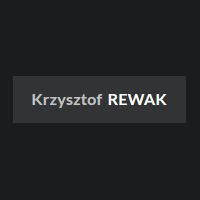
\includegraphics[width=.15\textwidth]{../_template/rewak.png}
		}
	\end{figure}

\end{frame}

\end{document}
